\documentclass{article}
\usepackage[fleqn]{amsmath}
\usepackage{amssymb}
\usepackage{algorithm}
\usepackage{algpseudocode}
\usepackage{algorithmicx}
\usepackage{enumitem}
\usepackage{listings}
\usepackage{xcolor}
\usepackage{apacite}
\usepackage{svg}
\usepackage{placeins}

\lstset{
	language=C++,
	backgroundcolor=\color{black!5},
	basicstyle=\footnotesize,
}

\title{CAB302 - Assignment 1}
\author{Luke Josh   }
\begin{document}
\bibliographystyle{apacite}
\maketitle\pagebreak
\tableofcontents
\pagebreak

\section{Introduction}
    \subsection{Background}
    Insertion sort is an algorithm that takes an input of an unsorted (or sorted) list of numbers, and rearrangesthem into asscending order. It belongs to a group of algorithms known as sorting algorithms, but is by far from the best.There are a number of more complex algorithms that can work much faster (especially as the size of the array increases),however, it is extremely simple, easy to implement, and a great tool to teach computer science students about algorithms and complexity.\\
    The algorithm can be thought of as seperating the array into two subarrays, one that is sorted, and one that isn't. Traditionaalgorithm begins at theleftmost element - splitting the array into the far left element, and every else to the right. Initially, the first element of tis sorted -as there is nothing to compare it to. The remaining unsorted elements are then itteratively comparedto the sorted elements, and are placed into the index in which they belong. The process is often described as how a human would sort a hand of cards.An implementation of the algorithm is included below:\\

    \subsection{Pseudo-code of the Algorithm}
        \begin{algorithmic}[1]  
            \Function{InsertionSort}{$A[0..n-1]$}
                \For{$i \leftarrow 1$ \bf{to} $n - 1$}
                    \State{$v \leftarrow A[i]$}
                    \State{$j \leftarrow i - 1$}
                    \While{$j \geq 0$ \bf{and} $A[j] > v$}
                        \State{$A[j + 1] \leftarrow A[j]$}
                        \State{$j \leftarrow j - 1$}
                    \EndWhile
                    \State{$A[j + 1] \leftarrow v$}
                \EndFor
            \EndFunction
        \end{algorithmic}

    \subsection{Algorithm in words}
        In words, the algorithm can be expressed as follows:
        \begin{enumerate}[itemsep=0mm]
            \item Take the nth element of the array, starting from the 2nd element, call this the subject element
            \item Compare the nth element with the n-1th element (the element to the left)
            \item If the element to the left is larger than the subject element, swap the two elements
            \item Else, if there is no item to the left, or the item to the left is less than the subject element, do nothing, and proceed along the array
            \item Repeat for all elements of the array
        \end{enumerate}

    \subsection{An Example}
        This can be observed in a simple example, take the array $A=[1, 3, 4, 2, 0]$ - the algorithm would observed the following steps:

        \begin{enumerate}[itemsep=0mm]
            \item Take the Second element, $v=1$, the element to the left is lower, continue
            \item Take the third element, $v=3$, the element to the left is greater, so call the third element, 4, the subject element
            \item Perform $A[j + 1] \leftarrow A[j]$, which becomes $A[3] \leftarrow A[2]$, thus $A=[1, 3, 4, 4, 0]$
            \item Repeat this operation along the list, until the item to the left is no longer less than the subject element: $A=[1, \mathbf{3}, 3, 4, 0]$
            \item Now, as the previous element is not less than the subject element, instead of making the element equal to the one before it ($A[j + 1] \leftarrow A[j]$), we set the element to be the subject element($A[j + 1] \leftarrow      v$), thus, $A=[1, 2, 3, 4, 0]$
            \item Repeat the process for the last element, which yields $A=[0, 1, 2, 3, 4]$
        \end{enumerate}

\section{Theoretical Analysis}
    \subsection{Basic Operation}
        To analyse the efficiency of insertion sort, we must define the \textit{basic operation} of the algorithm. The basic operation is said to be the operation which has the most influence on the running time of the algorithm, which can usually be said to be the operation which is performed with the highest frequency. The operation, in this case, is the check $A[j] > v$. This check is performed more than any other in the algorithm.
    \subsection{Best Case}
        The best case efficiency for insertion sort is when the array is already sorted. For a sorted array, $A = [a_1, a_2, ..., a_n]$, each element $a_{i} \geq a_{i-1} \forall i \in [2, 3, ... n]$, and thus, each element that is to be sorted will only check against the element to it's left. Therefore, for a sorted array $A$ with $n$ elements, the number of comparisons that must be performed is $c = n - 1$, giving the algorithm a running time of $\Theta(n)$.
    \subsection{Worst Case}
        The worse case efficiency for insertion sort is for an array that is sorted in descending order. An array of this fashion will require a check for each value to the left of each value in the array. For example, if we have the array $A=[5, 4, 3, 2, 1]$, for the first value to be checked, $v = 4$, we must check that the value to the left is not greater, so, 1 comparison. For the second value to be checked, $v = 3$, we must check the two values to the left, so 2 comparisons. It continues in this fashion, and we have the number of comparisons, $c = 1 + 2 + 3 + 4$. Extending this to an array $B=[b_1, b_2, b_3, ..., b_n]$, the number of comparisons, c becomes

        \begin{align}
            & c = 1 + 2 + 3 + ... + (n - 1) \\
            & c = \sum_{j = 1}^{n - 1} j \\
            & c = (\sum_{j = 1}^{n} j) - n\\
            & c = \frac{n(n + 1)}{2} - n \\
            \therefore{} & c = \frac{n(n - 1)}{2}
        \end{align}

    \subsection{Average Case}
        Assuming an array $A = [a_1, a_2, ..., a_n]$ who's values could take any possible permutation of the natural numbers, the \'average case\' number of basic operations can be calculated. In this case, we can assume that since all elements are randomly selected from the set of natural numbers, that each element is equally likely to be greater than or less than each other element, and from that, we can state that for each element, half of the elements to the left will have to be checked before one is found that is larger than it, on average. Thus, we can state that for each element $a_i$ in $A$, approximately $\frac{i}{2}$ comparisons must be made:

        \begin{align}
            & c = \sum_{j = 1}^{n - 1} \frac{j}{2} \\
            & c = (\sum_{j = 1}^{n} \frac{j}{2}) - \frac{n}{2}\\
            & c = \frac{(\sum_{j = 1}^{n} j)}{2} - \frac{n}{2}\\
            & c = \frac{n(n + 1)}{4} - \frac{n}{2}
        \end{align}

        The average case efficiency is much more accurately calculated and quoted by McQuain~\cite{McQuain2000}, as $\frac{n^2}{4}$. Both of these values for the average case efficiency give the algorithm a running time of $\Theta(n^2)$.

\section{Methodology, Tools and Techniques}
    The following sections regarding the tests that were performed to test the algorithm were run on relatively powerful personal computer, with the following specifications:
    \begin{itemize}
        \item Intel Core i7 @ 2.40GHz
        \item 8GB DDR3 Memory @ 1600MHz
        \item Running Ubuntu 14.04 (64 bit)
    \end{itemize}

    All tests were written in C++, and were compiled using the CLion IDE. Average case tests are performed by generating generating pseudo-random arrays using the c++ rand functions. Graphs that are shown were produced by reading outputs into a Python script using the matplotlib library~\cite{Hunter2007}.

    This report was typeset and formatted using the \LaTeX\  package.

\section{Experimental Analysis}
    \subsection{Tests}
        A number of tests can be applied to the operation on this algorithm to test it's efficiency, and how well it conforms to the theoretical analysis above. This report will detail a count of the number of basic operations performed to sort an array, along with the time taken to sort an array. All referenced figures are included in Appendix A.

    \subsection{Number of Operations}
        The number of basic operations for the Insertion Sort algorithm is a well defined concept, and can be quantitatively measured and compared to a literature value. The following sections outline results from several tests performed using the included code. Referring to the pseudo code in Section 1.2, we would initialise at a counter at zero at the start of the algorithm, and increment it
        \subsubsection{Best Case}
            Recall from above that the best case running time occurs when an array $A = [a_1, a_2, ..., a_n]$ is already sorted such that $a_n \leq a_{n+1} \forall\ n \in [1, 2, ..., n - 1]$, and that it is expected to run with n - 1 operations. To test this, we can generate arrays that are sorted, and then measure the number of operations required to complete the algorithm. To ensure that the relation is indeed correct, the expected and actual number of basic operations will be calculated for arrays of size 2 through 1000. Two graphs have been produced for this test - one that displays the data that was measured (Figure 1), and another that shows the expected output (Figure 2), these have been included separately to highlight the fact that the two data are exactly the same.

        \subsubsection{Worst Case}
            The worst case for Insertion Sort was said to be an array $A = [a_1, a_2, ..., a_n]$, sorted in reverse order such that $a_n \geq a_{n+1} \forall\ n \in\ [1, 2, ..., n - 1]$. The expected number of operations here was said to be $\frac{n(n - 1)}{2}$. To test this, data is again generated, but this time in descending order. To ensure correctness, it has also been tested on arrays of size 2 through 1000. For this test case, only one image was shown, displaying the expected output and the actual output on the same graph. Barely any distinction is visible between these two lines, indicating that our expected number of operations is indeed correct. The graphs have been included as Figure 3.

        \subsubsection{Average Case}
            The average case for Insertion Sort was said to be an array of numbers, each number being equally likely to be greater than or less than each other number, the expected number of operations was quoted to be $\frac{n^2}{4}$. To test the expected value of basic operations, arrays of varying sizes were generated, with each element being a random number between zero and twice the number of elements. Twice the number of elements was chosen just so that there are less occurrences of duplicate values, and that the array has a greater chance of entropy, and thus, a more accurate ``average'' result. We generate a number of these arrays of each size, calculate the number of operations, and take the average - this is to ensure functional correctness, and to get a better reading of the average case. Arrays of size 2 through 1000 were tested, taking an average of 10 generations each time.\\

            To calculate the random value, the \texit{rand()} function can be used, which generates a random number between zero and some (unnecessarily high) predefined integer. To generate a random number in a specified range, we can use the modulo operator to reduce the generated number down to a limit of the desired maximum value, less the minimum value, and then add the minimum value. In c++, this looks like \texit{rand() \% (upper - lower + 1) + lower} - which will generate a value somewhere between \textit{lower} and \textit{upper}.\\

            A graph has been included as Figure 4 showing the expected and theoretical data for this test. Unlike the previous trials on best and worst case data, these trials will not produce the exact expected value each time, but when averaged, will tend towards the expected value. This can be verified visually, the blue dots representing a measured number of operations for a particularly sized array does not form a seemingly continuous line like the other tests.

    \subsection{Processing Time}
        The time taken to run the run the algorithm can be simply calculated by the difference between the time at the start of the algorithm, and the time at the end of the algorithm. In c++, this can be done using the \texit{clock()} function. The clock function returns the number of ticks that have elapsed since the program was executed - we can couple this with the CLOCKS_PER_SECOND constant to determine the number of seconds that have elapsed. To find the running time of the algorithm, we find the number of ticks it took the program to run, by subtracting the number of ticks at the start of the program from the number of ticks at the successful completion of the program, divided by the CLOCKS_PER_SECOND constant.\\

        Although no time can be calculated to compare against, it can be known that a computer will be able to very quickly process these algorithms. In fact, the algorithm will process so quickly, that the time measured may not be entirely accurate or useful to look at. To combat this, rather than testing the time it takes for a single array to be sorted, we test the time it takes to sort a large number of arrays of that size, and find the average.

        \subsubsection{Best Case}
            Like in the operations count, sorted arrays of sizes 2 through 1000 will be generated and sorted. However, to get a better reading, the average will be taken over 100 samples of each size.

\section{Appendices}
    \subsection{Appendix A - Graphs}
        \begin{figure}[h]
            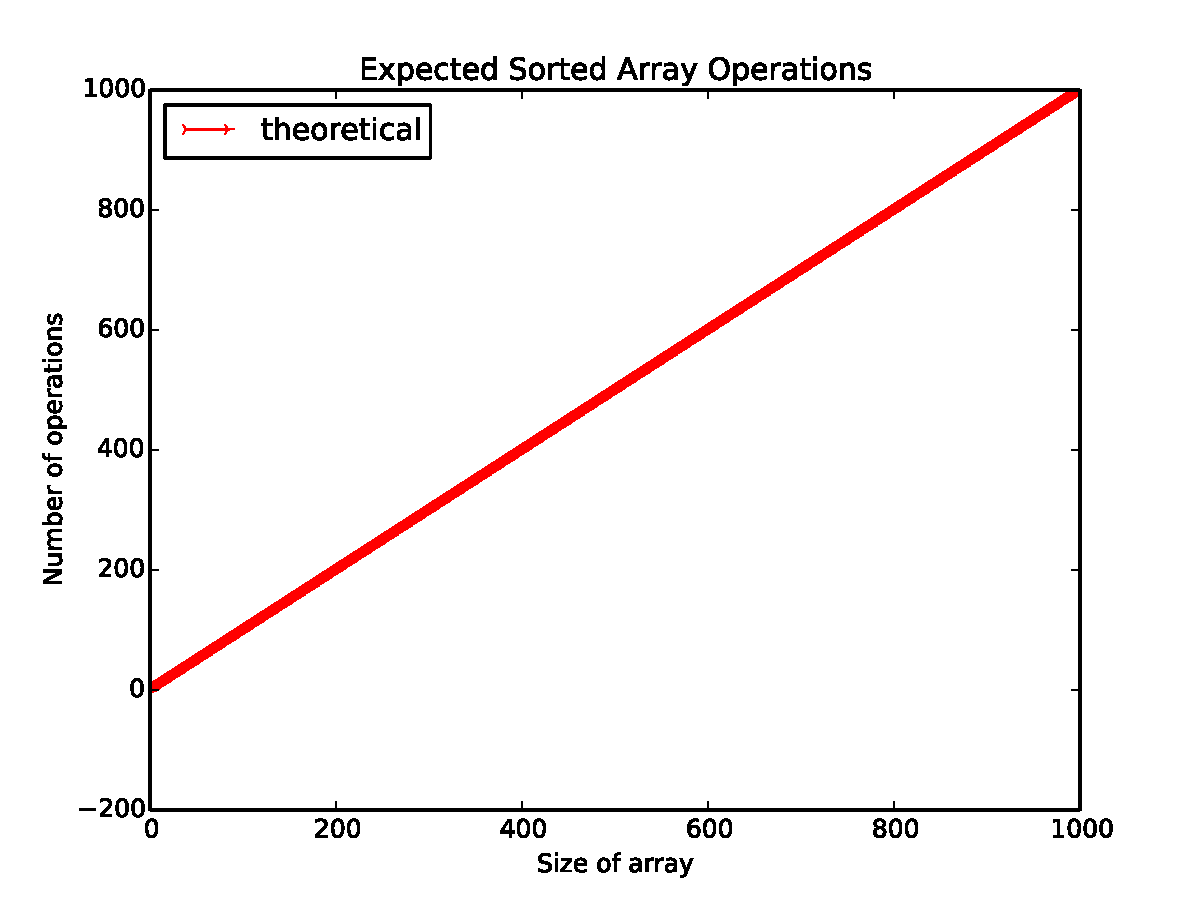
\includegraphics[width=\textwidth, height=0.4\textheight]{sorted_array_basic_operation_count_expected}
            \caption{Expected number of operations for sorted arrays of size 2 through 1000}
        \end{figure}
        \begin{figure}[h]
            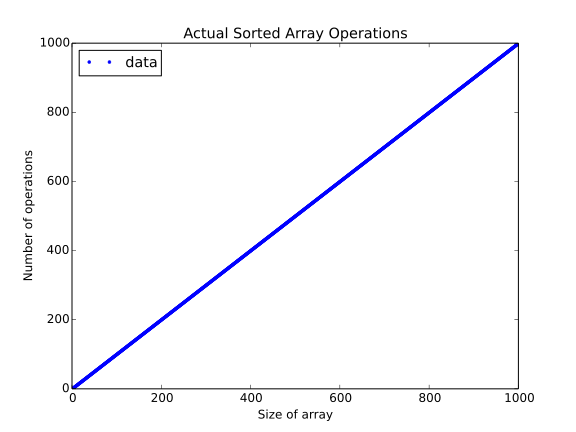
\includegraphics[width=\textwidth, height=0.4\textheight]{sorted_array_basic_operation_count_data}
            \caption{Recorded number of operations for sorted arrays of size 2 through 1000}
        \end{figure}
        \begin{figure}[h]
            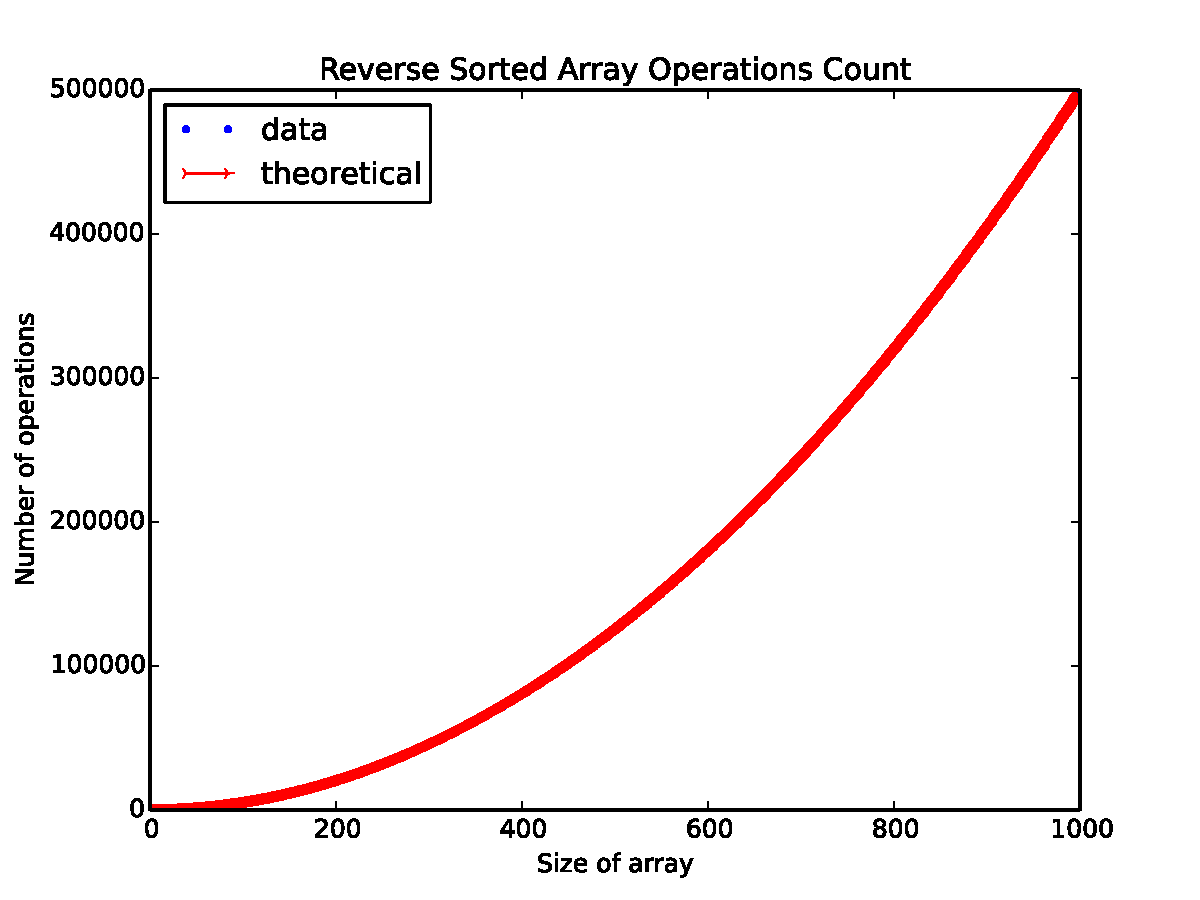
\includegraphics[width=\textwidth, height=0.4\textheight]{reverse_sorted_array_basic_operation_count}
            \caption{Number of operations on reversed sorted arrays of size 2 through 1000}
        \end{figure}
        \begin{figure}[h]
            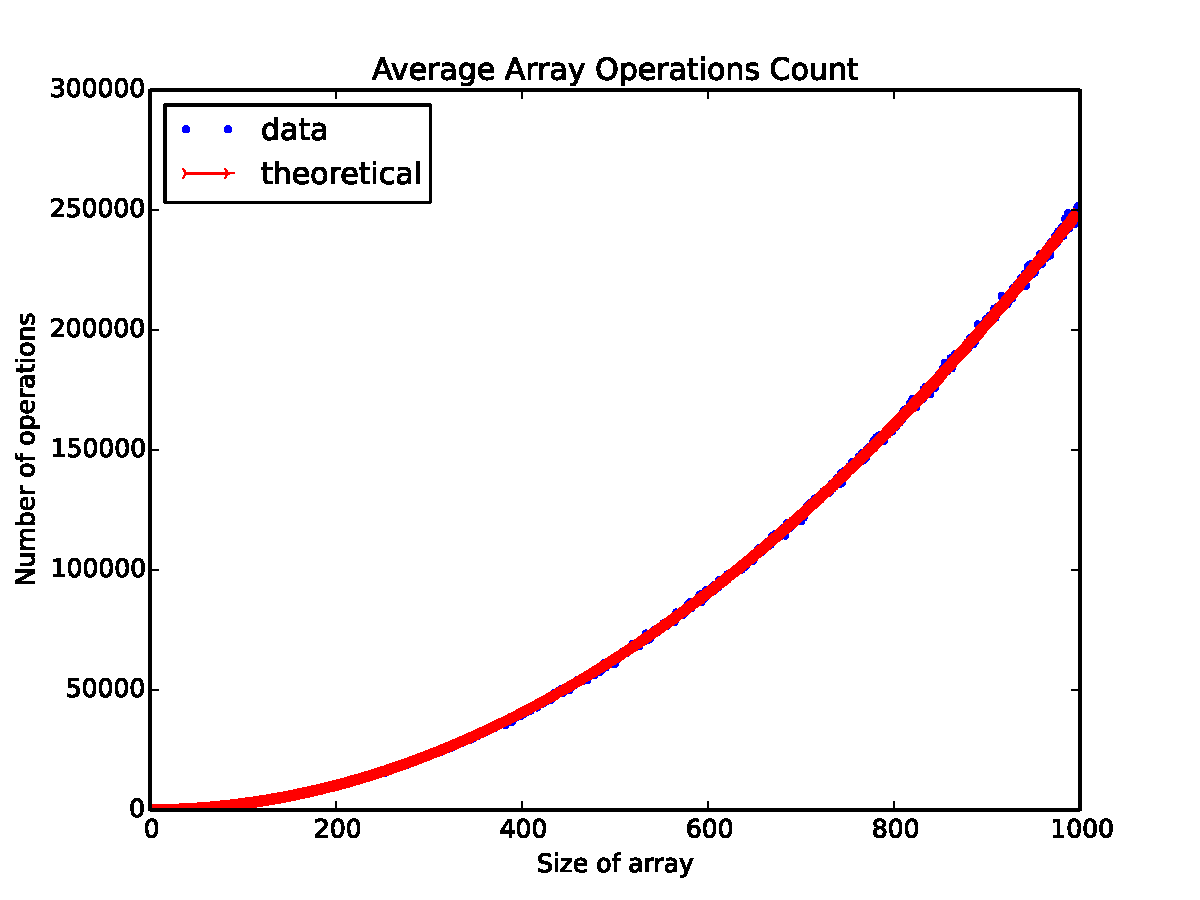
\includegraphics[width=\textwidth, height=0.4\textheight]{random_basic_operation_count}
            \caption{Number of operations on average arrays, for arrays of size 2 through 1000, averaged over 10 trials}
        \end{figure}
    \FloatBarrier

    \subsection{Source Code}
        \lstinputlisting{main.cpp}\newpage

\section{Bibliography}
    \bibliography{bibliography}

\end{document}